
\documentclass{beamer}
\usetheme{Wrexham}  
\usepackage{graphicx}
\usepackage{algorithm}
\usepackage{algorithmic}
\usepackage{caption}
\usepackage{subcaption}
\graphicspath{{./figures/}}
\begin{document}
\title{Magic, Syphilis and C.S.I}
\subtitle{A friendly introduction to compressive sensing.}
\author{Rhian Davies}
\titlegraphic{ 
\includegraphics[height=.2\textheight]{logoEPSRC.png} \hspace{3cm} 
\includegraphics[height=.2\textheight]{logoSTORi.png}}
%\titlegraphic{
\includegraphics[height=.2\textheight]{logoEPSRC.png}}
\date{\today}

\begin{frame}[plain] 
  \titlepage
\end{frame}
%%%%%%%%%%%%%%%%%%%%%%%%%%%%%%%%%%%%%%%%%%%%%%%%%%%%%%%%%%%%%%%%%%%%%%%%%%%%%%%%%%%%%%%%%%%%%%%%%%%%%%%%
%%%%%%%%%%%%%%%%%%%%%%%%%%%%%%%%%%%%%%%%%%%%%%%%%%%%%%%%%%%%%%%%%%%%%%%%%%%%%%%%%%%%%%%%%%%%%%%%%%%%%%%%
%%%                                             MAGIC TRICK                                          %%%
%%%%%%%%%%%%%%%%%%%%%%%%%%%%%%%%%%%%%%%%%%%%%%%%%%%%%%%%%%%%%%%%%%%%%%%%%%%%%%%%%%%%%%%%%%%%%%%%%%%%%%%%
%%%%%%%%%%%%%%%%%%%%%%%%%%%%%%%%%%%%%%%%%%%%%%%%%%%%%%%%%%%%%%%%%%%%%%%%%%%%%%%%%%%%%%%%%%%%%%%%%%%%%%%%
%

\begin{frame}
  \begin{figure}[h]
    \centering
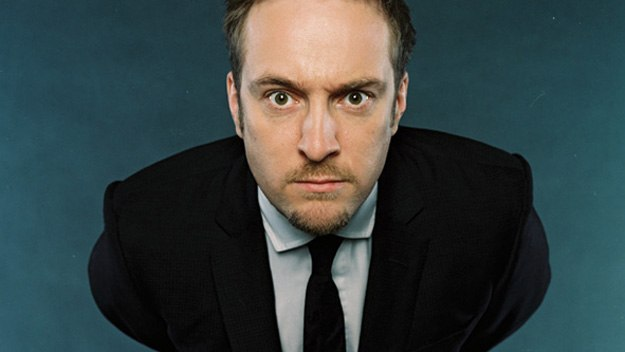
\includegraphics[height = 6cm]{derrenbrown.jpg}    
  \end{figure}
\end{frame}

\begin{frame}
  \begin{table}[h]
    \centering
    \begin{tabular}{|c c c c c c c c|}\hline
      2  & 3  & 6  & 7  & 10 & 11 & 14 & 15 \\
      18 & 19 & 22 & 23 & 26 & 27 & 30 & 31 \\
      34 & 35 & 38 & 39 & 42 & 43 & 46 & 47 \\
      50 & 51 & 54 & 55 & 58 & 59 & 62 & 63 \\ \hline
    \end{tabular}
  \end{table}
\end{frame}
%
\begin{frame}
  \begin{table}[h]
    \centering
    \begin{tabular}{|c c c c c c c c|}\hline
     16 & 17 & 18 & 19 & 20 & 21 & 22 & 23 \\
     24 & 25 & 26 & 27 & 28 & 29 & 30 & 31 \\
     48 & 49 & 50 & 51 & 52 & 53 & 54 & 55 \\
     56 & 57 & 58 & 59 & 60 & 61 & 62 & 63 \\ \hline
    \end{tabular}
  \end{table}
\end{frame}
%
\begin{frame}
  \begin{table}[h]
    \centering
    \begin{tabular}{|c c c c c c c c|}\hline
      8  & 9  & 10 & 11 & 12 & 13 & 14 & 15 \\
      24 & 25 & 26 & 27 & 28 & 29 & 30 & 31 \\
      40 & 41 & 42 & 43 & 44 & 45 & 46 & 47 \\
      56 & 57 & 58 & 59 & 60 & 61 & 62 & 63 \\ \hline
    \end{tabular}
  \end{table}
\end{frame}
%
\begin{frame}
  \begin{table}[h]
    \centering
    \begin{tabular}{|c c c c c c c c|}\hline
   1  & 3  & 5  & 7  & 9  & 11 & 13 & 15 \\
   17 & 19 & 21 & 23 & 25 & 27 & 29 & 31 \\
   33 & 35 & 37 & 39 & 41 & 43 & 45 & 47 \\
   49 & 51 & 53 & 55 & 57 & 59 & 61 & 63 \\ \hline
    \end{tabular}
  \end{table}
\end{frame}
%
\begin{frame}
  \begin{table}[h]
    \centering
    \begin{tabular}{|c c c c c c c c|}\hline
   4  & 5  & 6  & 7  & 12 & 13 & 14 & 15 \\
   20 & 21 & 22 & 23 & 28 & 29 & 30 & 31 \\
   36 & 37 & 38 & 39 & 44 & 45 & 46 & 47 \\
   52 & 53 & 54 & 55 & 60 & 61 & 62 & 63 \\ \hline
   \end{tabular}
  \end{table}
\end{frame}
%
\begin{frame}
  \begin{table}[h]
    \centering
    \begin{tabular}{|c c c c c c c c|}\hline
   32 & 33 & 34 & 35 & 36 & 37 & 38 & 39 \\
   40 & 41 & 42 & 43 & 44 & 45 & 46 & 47 \\
   48 & 49 & 50 & 51 & 52 & 53 & 54 & 55 \\
   56 & 57 & 58 & 59 & 60 & 61 & 62 & 63 \\ \hline
    \end{tabular}
  \end{table}
\end{frame}



%%%%%%%%%%%%%%%%%%%%%%%%%%%%%%%%%%%%%%%%%%%%%%%%%%%%%%%%%%%%%%%%%%%%%%%%%%%%%%%%%%%%%%%%%%%%%%%%%%%%%%%
%%%%%%%%%%%%%%%%%%%%%%%%%%%%%%%%%%%%%%%%%%%%%%%%%%%%%%%%%%%%%%%%%%%%%%%%%%%%%%%%%%%%%%%%%%%%%%%%%%%%%%%%
%%%                                             END                                                  %%%
%%%%%%%%%%%%%%%%%%%%%%%%%%%%%%%%%%%%%%%%%%%%%%%%%%%%%%%%%%%%%%%%%%%%%%%%%%%%%%%%%%%%%%%%%%%%%%%%%%%%%%%%
%%%%%%%%%%%%%%%%%%%%%%%%%%%%%%%%%%%%%%%%%%%%%%%%%%%%%%%%%%%%%%%%%%%%%%%%%%%%%%%%%%%%%%%%%%%%%%%%%%%%%%%

\begin{frame}
  \frametitle{Syphilis in World War II}

\begin{columns}
\begin{column}{.48\textwidth}

  \begin{itemize}
  \item US PHS study WWII
  \item Rob Dorfman ``The detection of defective members of large populations.''  1943
  \item We can combine $M$ blood samples together and test a combined sample to see if at least one recruit in the sample has syphilis. 
  \item If negative we have ``saved'' $M-1$ tests. 
  \item If positive, we have ``wasted'' a test. 
  \end{itemize}

%Syphilis is a sexually transmitted infection. 
%During World War II US PHS wanted a study
%3 an economist at heart working in the Price stas branch of reaserch at Washington D.C.
%Took the theory and check probailistic properties and invented group testing (Annals of Mathematical Statistics)
%If $M$ reaches 10, the syphilis 
%Tests were expensive, testing indivually seemed silly. 
%Estimated that 10\% may have syphilis. 
\end{column}
%\hfill

\begin{column}{.48\textwidth}
  \begin{figure}[h]
   % \centering

\includegraphics[height = 6cm]{unclesam.jpg}    

  \end{figure}

\end{column}%
\end{columns}

\end{frame}


\begin{frame}
  \frametitle{The coin puzzle}
 \begin{figure}
    \href{http://nrich.maths.org/5796}
         {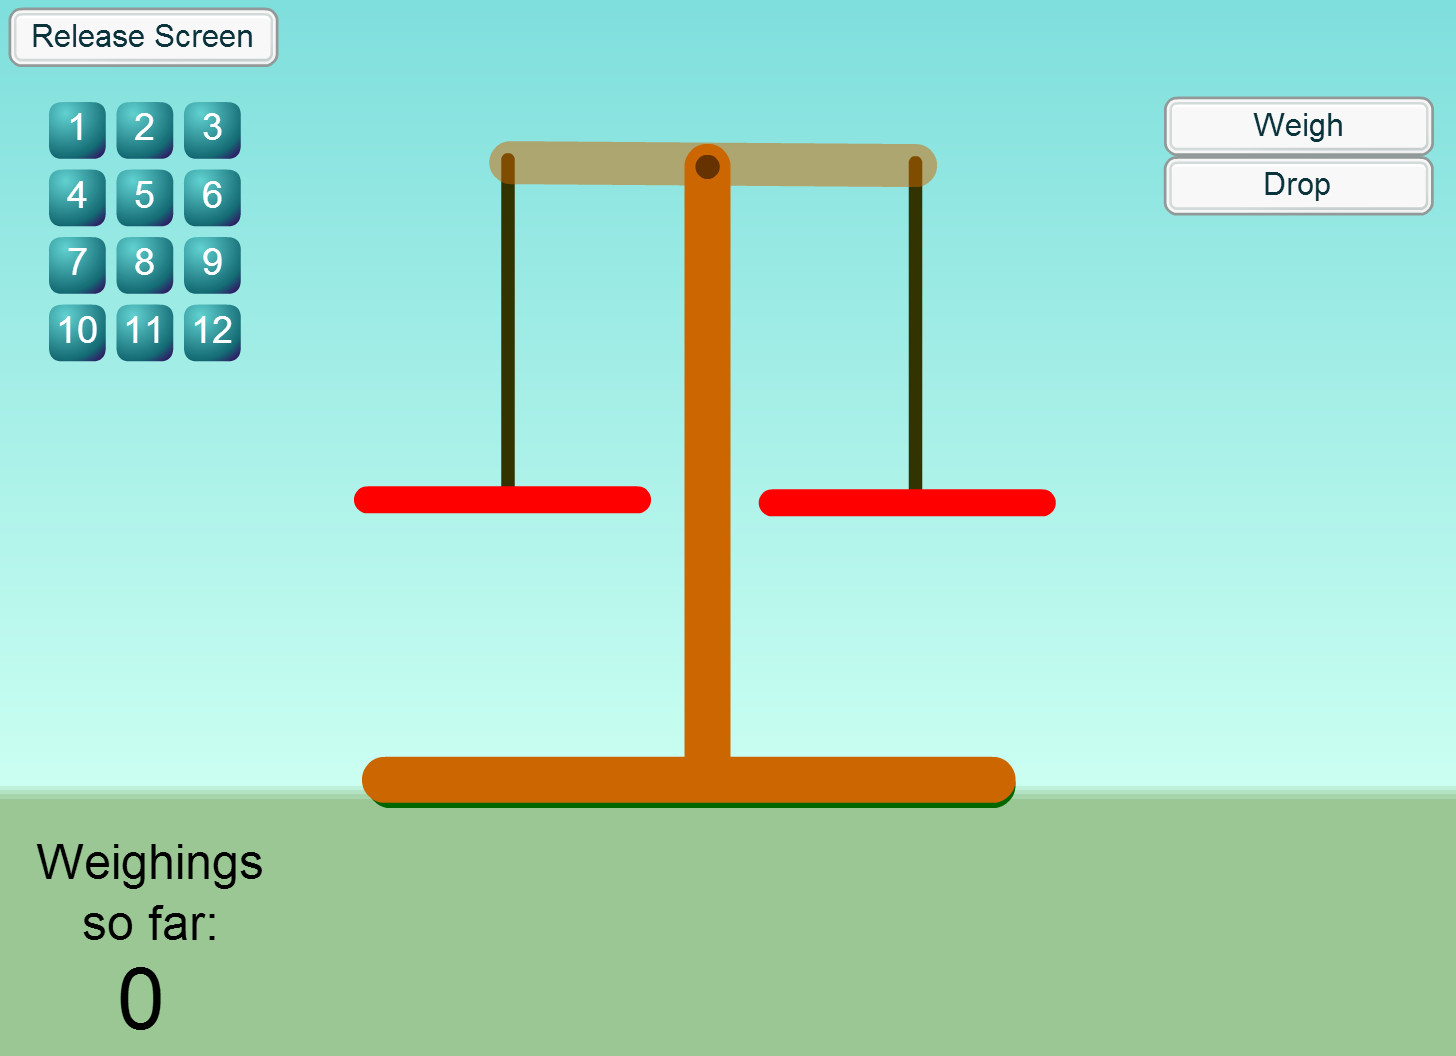
\includegraphics[height = 6cm]{balance}}
  \end{figure}
\end{frame}

  \begin{frame}
    \frametitle{Non-adaptive solution}
    
 \begin{table}[h]
    \centering
    \begin{tabular}{|c c c c| c | c c c c|}
     1 & 2 & 3 & 4 & vs & 5 & 6 & 7 & 8 \\
     1 & 4 & 8 & 9 & vs & 2 & 3 & 11 & 12 \\
     3 & 7 & 9 & 12 & vs & 1 & 2 & 5 & 10\\
    \end{tabular}
  \end{table}

  \end{frame}

  \begin{frame}
    \frametitle{What do these group testing examples have in common?}


   \begin{itemize}
   \item Sparsity
   \item Testing in subsets / Reduced number of measurements
   \item Non adaptive measurements
   \item Decoding procedure
   \end{itemize}
  \end{frame}

  \begin{frame}
    \frametitle{Compressive Sensing}
    
    \begin{itemize}
    \item $M \times N$ measurement matrix $\Phi$ $(M \ll N)$
    \item Signal $x \in R^N$ which is sparse (contains k nonzero entries).
    \item Identify the location of $k$ elements using $y = \Phi x$ measurements
    \item How small can we make M and still recover x using only y?
    \end{itemize}
  \end{frame}

\begin{frame}
\frametitle{The encoding process.} % Assume that the signal of interest $\pmb{x}$ is of length N.
\begin{figure}[h]
        \centering
        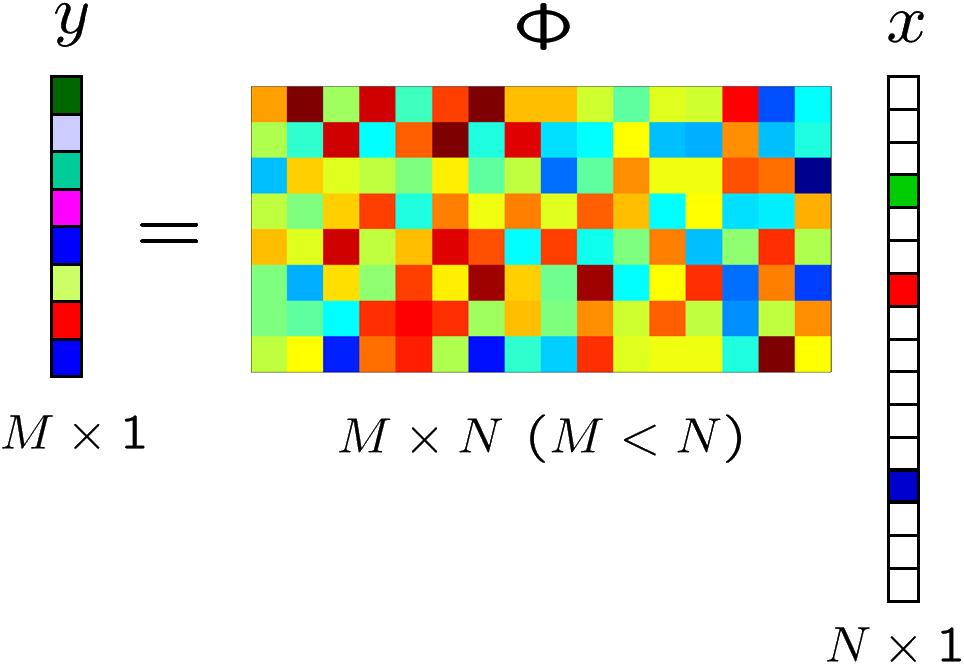
\includegraphics[width = 8cm]{csss}
        \caption{CS measurement process, courtesy of Volkan Cevher.}
      \end{figure}
\end{frame}

\begin{frame}
  \frametitle{ Measurement Matrix $\Phi$: Null space condition}
We require that the signal $\boldsymbol{x}$ can be uniquely reconstructed. It is possible to show that this will hold true if the null space $\mathcal{N}(\boldsymbol{\Phi})$ does not contain any vectors in $\Sigma_{2K}$. 
\begin{equation*}
  \mathcal{N}(\boldsymbol{\Phi}) = (\boldsymbol{z}:\boldsymbol{\Phi}\boldsymbol{z}=0). 
\end{equation*}

In order to preserve $\boldsymbol{x} \in \Sigma_K$, it is required $\boldsymbol{\Phi x} \neq \boldsymbol{\Phi x^{\prime}} \; \forall  \boldsymbol{x^{\prime}} \in \Sigma_K$, because  if $\boldsymbol{\Phi x} = \boldsymbol{\Phi x^{\prime}}$ it would be impossible to distinguish $\boldsymbol{x}$ from $\boldsymbol{x^{\prime}}$ based only on $\boldsymbol{y}$. 
%Consider the case where $\boldsymbol{\Phi x} = \boldsymbol{\Phi x^{\prime}}$.
\begin{align*}
   \text{Consider,} \hspace{1cm} \boldsymbol{\Phi x} &= \boldsymbol{\Phi x^{\prime}} \\
& \Rightarrow \boldsymbol{\Phi}(\boldsymbol{x} - \boldsymbol{x^{\prime}}) = 0\\
&\Rightarrow (\boldsymbol{x} - \boldsymbol{x^{\prime}}) \in \Sigma_{2K}
\end{align*}

$\boldsymbol{\Phi}$ uniquely represents all $\boldsymbol{x} \in \Sigma_K \iff v \notin \mathcal{N}( \boldsymbol{\Phi}) \; \forall \boldsymbol{v} \in \Sigma_{2K}$. 
\end{frame}

\begin{frame}
  \frametitle{Measurement Matrix $\Phi$: Restricted Isometry Property}

  \begin{itemize}
  \item $\boldsymbol{y}$ may be corrupted by noise during the measurement process.

  \item Matrix $\boldsymbol{\Phi}$ satisfies the (RIP) of order $K$ if there exists a $\delta_K  \in (0,1)$ such that 
\begin{equation*}
  \label{eq:40}
  (1 - \delta_k)||\boldsymbol{x}||^2_2 \leq||\boldsymbol{\Phi} \boldsymbol{x}||^2_2 \leq (1 + \delta_k)||\boldsymbol{x}||^2_2,
\end{equation*}

for all $\boldsymbol{x} \in \sum_K = {\boldsymbol{x}:||\boldsymbol{x}||_0 \leq K} $. 


 \item  $\boldsymbol{\Phi}$ preserves the distance between any pair of $K$-sparse vectors.
\item This  gives a stronger guarantee of robustness against noise. 

\item Both of these conditions will hold true with high probability if $\boldsymbol{\Phi}$ is selected as a random matrix.
  \end{itemize}

\end{frame}

      \begin{frame}{Recovery of sparse transforms}
\label{recovery}
        \begin{itemize}
\item Solve $\boldsymbol{y} = \boldsymbol{\Phi x}$ , infinitely many solutions! Fat $\boldsymbol{\Phi}$ implies underdetermined system. 
\item We know that $\boldsymbol{x}$ was \textbf{sparse} 
       %   \item $\Delta(y, \Phi) = x$
%\item Ideally use the $\ell_0$ norm. 
\item What algorithms can we use to decode? 
\item Convex Optimisation or Greedy Algorithms or something else...?
        \end{itemize}

\hyperlink{l1}{\beamergotobutton{$\ell_1$ minimisation}}
\hyperlink{omp}{\beamergotobutton{Orthogonal Matching Pursuit}}
\end{frame}

\begin{frame}
  \frametitle{Traditional Image Acquisition}
  \begin{figure}[h]
    \centering
    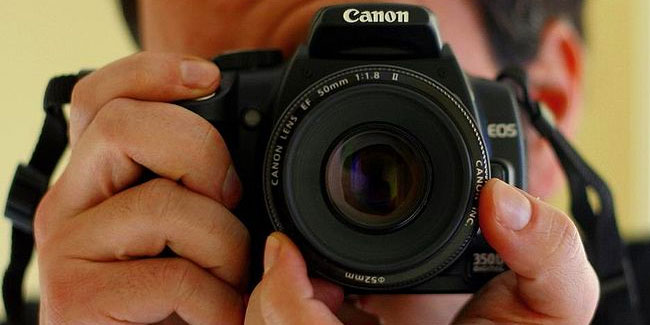
\includegraphics[width = 8cm]{camera.jpg}
  \end{figure}
  \begin{center}
We cannot use compressive sensing with this camera!    
  \end{center}

\end{frame}

 \begin{frame}
   \frametitle{The single pixel camera.}
   \begin{figure}[h]
     \centering
     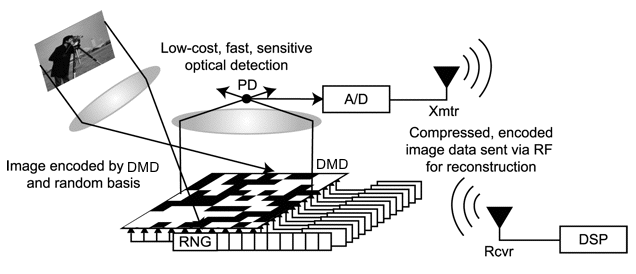
\includegraphics[width = 9cm]{spc}
     \caption{The single pixel camera}
   \end{figure}
 Doesn't acquire a single ray of light per pixel but rather a combination of rays of light (each coming from a different direction or spectral band or both) per pixel. To obtain back a picture that can be understood by the human eye, one needs the reconstruction methods mentioned earlier.
    \end{frame}

    \begin{frame}
      \frametitle{Digital micro-mirror device }
      \begin{figure}[h]
        \centering
        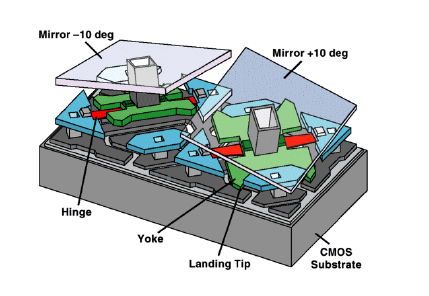
\includegraphics[width = 6cm]{DMD.png}
      \end{figure}
      \begin{itemize}
        \item Many very tiny tilt-able mirrors. 
        \item Each mirror can be positioned in two states. 
          \item A random number generator modulates the positions. 
            \item Therefore the light, can be reflected in two distinct directions. 
      \end{itemize}
    \end{frame}

    \begin{frame}
      \frametitle{Image Acquisition}
\begin{columns}
\begin{column}{.48\textwidth}
  \begin{itemize}
  \item Mathematically - calculating inner products
    \item Each set of mirror orientations = one measurement.
      \item Repeat $M$ times.
 \item Therefore SPC compresses and samples in the measurement process.
  \end{itemize}
\end{column}
%\hfill

\begin{column}{.48\textwidth}
  \begin{figure}[h]
   % \centering
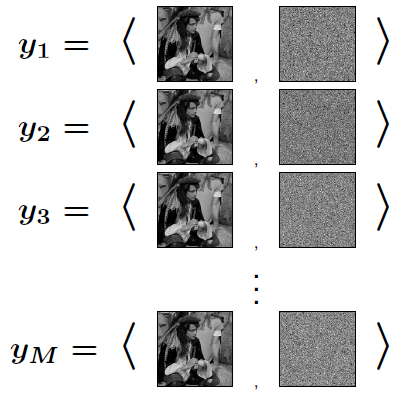
\includegraphics[height = 5cm]{sampling.png}    

  \end{figure}

\end{column}%
\end{columns}
      


    \end{frame}

    \begin{frame}
      \frametitle{Results from SPC}
      \begin{figure}[h]
        \centering
      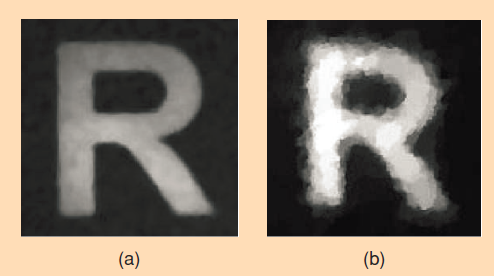
\includegraphics[width = 8cm]{result1.png}
  \caption{Reconstructed image taken with the SPC. (a) Conventional image of the target scene. (b) Reconstructed image with M = 1300 measurements. }

      \end{figure}
    \end{frame}

    \begin{frame}
      \frametitle{Why bother?}
      \begin{itemize}
      \item Data storage is cheap.
        \item We can store the information, so why bother?
          \item What about a fixed sensors on the moon?
            \item Scenarios where we need simplicity at the sensor, complexity at the analysis hub. 
      \end{itemize}
    \end{frame}

  \begin{frame}
    \frametitle{Compressive Sensing is not...}
 \begin{figure}
    \href{http://www.youtube.com/watch?v=LhF_56SxrGk}
         {
\includegraphics[height = 6cm]{csi}}
  \end{figure}
    
  \end{frame}

  \begin{frame}
    \frametitle{Any Questions?}
      \begin{figure}[h]
  \centering
  
\includegraphics[height=4cm]{questions.jpg}
 \end{figure} 
  \end{frame}

\begin{frame}
  \frametitle{Sparsity and wavelet transformation}
Achievable resolution is dependant on the information content of the image. If an image has low information content  it is said to be sparse and can be perfectly reconstructed from a small number of measurements. 

\bf{Nearly all real world images exhibit this sparsity property when transformed using a wavelet basis.}

  \begin{figure}[h]
    \centering
    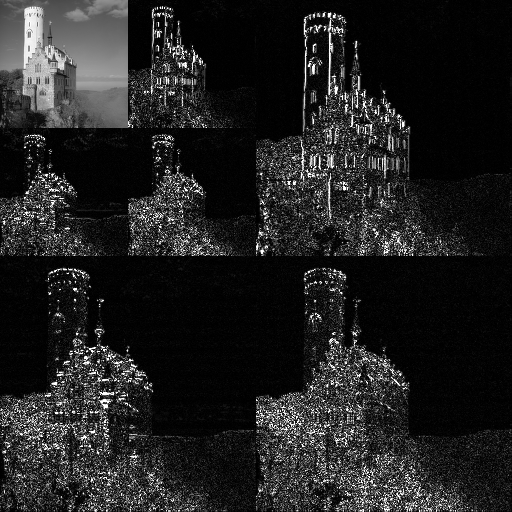
\includegraphics[height = 4cm]{wavelets}
    \caption{Wavelet transform}
    \label{fig:wavelet}
  \end{figure}

Note that most of the pixels here are black indicating low information content.
 \end{frame}


\begin{frame}
  \frametitle{Using $\ell_1$ minimization to promote sparsity}
\label{l1}

\begin{equation*}
\label{eq:57}
  \|\boldsymbol{x}\|_1 = \sum_{i=1}^{N}|x_i|
\end{equation*}

Originally used in geophysics to aid detection of sparse spike trends in earthquake data, optimisation based on the $l_1$ norm can closely approximate compressible signals with high probability.  
\begin{equation*}
  \label{eq:4}
  \min_{\boldsymbol{x}} ||\boldsymbol{x}||_1 \text{ subject to } \boldsymbol{y} = \boldsymbol{\Phi} \boldsymbol{x}.
\end{equation*}
\hyperlink{recovery}{\beamergotobutton{Recovery Algorithms}}

\end{frame}

\begin{frame}{Orthogonal Matching Pursuit}
\label{omp}
\begin{algorithm}[H]
%\caption{Orthogonal Matching Pursuit}  
\begin{algorithmic}
\STATE{Define the columns of $\boldsymbol{\Phi}$ to be $\varphi_1, \varphi_2, \hdots, \varphi_N$.}% each of length $M$.}
\REQUIRE $\boldsymbol{r_0} = \boldsymbol{y}, \Lambda_0 = \emptyset$ and iteration counter $i = 1$
\FOR{$i < T$} % \COMMENT{T is the maximum iteration count.}
 \STATE  $\lambda_t = \text{argmax }_{j=1,\hdots,N}|<r_{t-1}, \varphi_j>|$ \\  \COMMENT{Find the index for the column of $\Phi$ with the greatest contribution.}
 \STATE  $\Lambda_t = \Lambda_{t-1} \cup {\lambda_t}$, $\Phi_t = [\boldsymbol{\Phi_{t-1}}, \varphi_{\lambda_t}]$ \\ \COMMENT{Keeps track of the columns used.}
\STATE   $\boldsymbol{x_t} = \text{argmin}_{\boldsymbol{x}} || \boldsymbol{y} - \boldsymbol{\Phi_t} \boldsymbol{x}||_2$  \\ \COMMENT{Updates the signal estimate.}
\STATE  $\boldsymbol{r_t} =  \boldsymbol{y} - \boldsymbol{\Phi_t} \boldsymbol{x_t}$ \\ \COMMENT {Updates the measurement residual.}
\ENDFOR
\RETURN  $\boldsymbol{\hat{x}}$
\end{algorithmic}
\end{algorithm}
\hyperlink{recovery}{\beamergotobutton{Recovery Algorithms}}


\end{frame}


 \end{document}


%%%%%%%%%%%%%%%%%%%%%%%%%%%%%%%%%%%%%%%%%%%%%%%%%%%%%%%%%%%%%%%%%%%%%%%%%%%%%%%%%%%%%%%%%%%%%%%%%%%%%%%%%%%%%%%%%%%%%%%%%%%%%%%%%%%
%%%%%%%%%%%%%%%%%%%%%%%%%%%%%%%%%%%%%%%%%%%%%%%%%%%%%%%%%%%%%%%%%%%%%%%%%%%%%%%%%%%%%%%%%%%%%%%%%%%%%%%%%%%%%%%%%%%%%%%%%%%%%%%%%%%
%%%%%%%%%%%%%%%%%%%%%%%%%%%%%%%%%%%%%%%%%%%%%%%%%%%%%%%%%%%%%%%%%%%%%%%%%%%%%%%%%%%%%%%%%%%%%%%%%%%%%%%%%%%%%%%%%%%%%%%%%%%%%%%%%%%
%%%%%%%%%%%%%%%%%%%%%%%%%%%%%%%%%%%%%%%%%%%%%%%%%%%%%%%%%%%%%%%%%%%%%%%%%%%%%%%%%%%%%%%%%%%%%%%%%%%%%%%%%%%%%%%%%%%%%%%%%%%%%%%%%%%
 


 \begin{frame}{Sparsity}    

\begin{figure}
        \centering
        \begin{subfigure}[b]{0.4\textwidth}
                \centering
                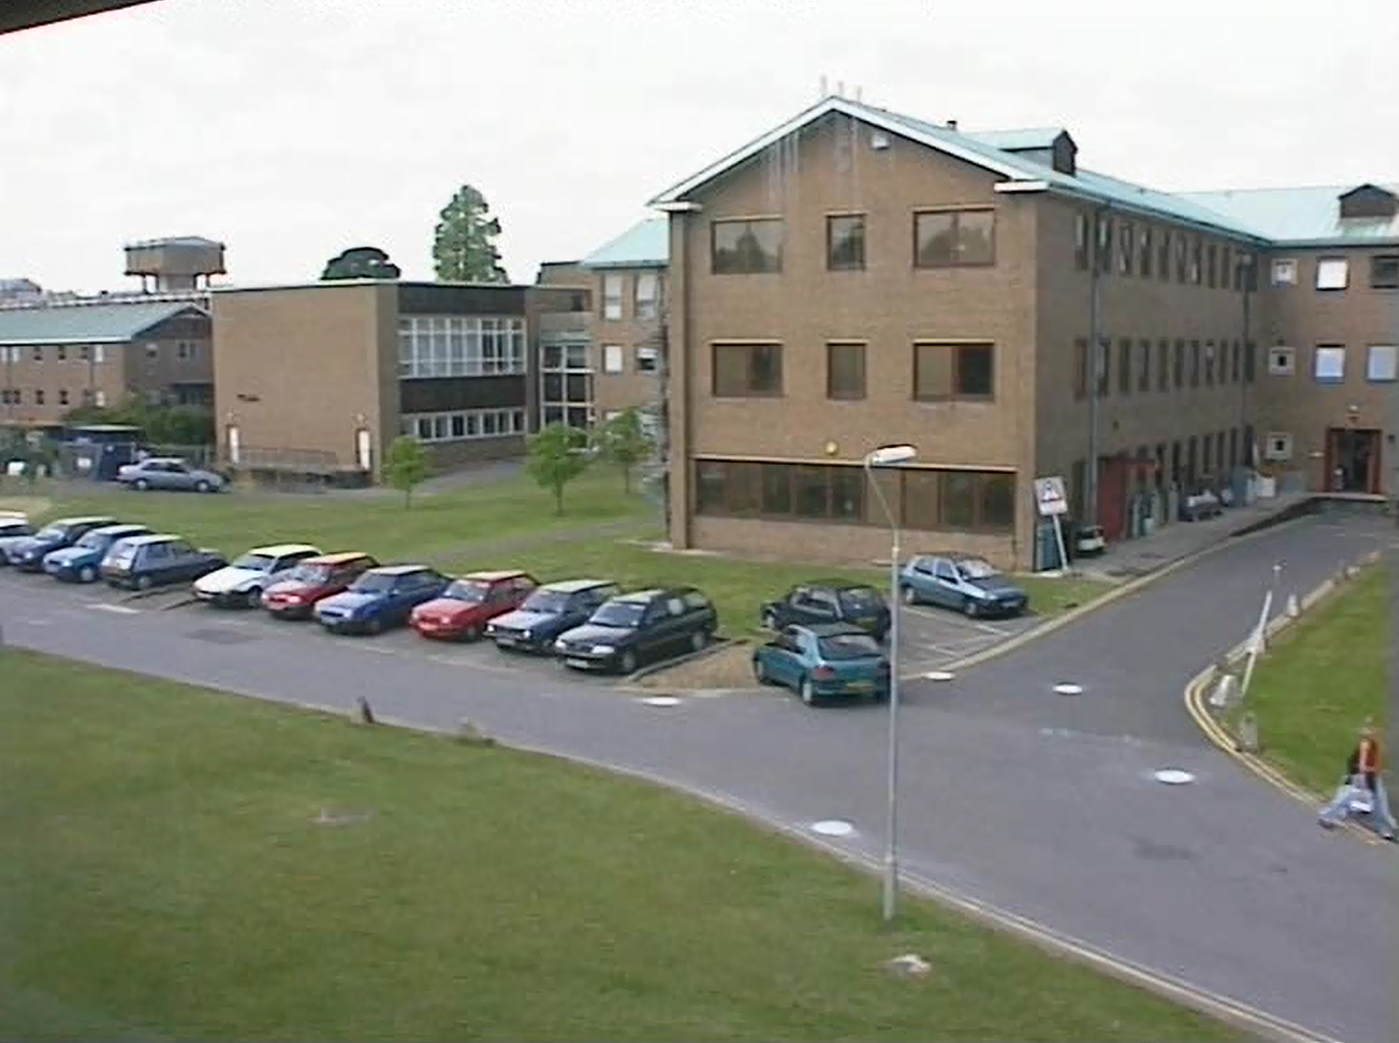
\includegraphics[width=\textwidth]{camReal}
                \caption{Test frame}
               % \label{fig:gull}
        \end{subfigure}%
        ~ %add desired spacing between images, e. g. ~, \quad, \qquad etc.
          %(or a blank line to force the subfigure onto a new line)
        \begin{subfigure}[b]{0.4\textwidth}
                \centering
                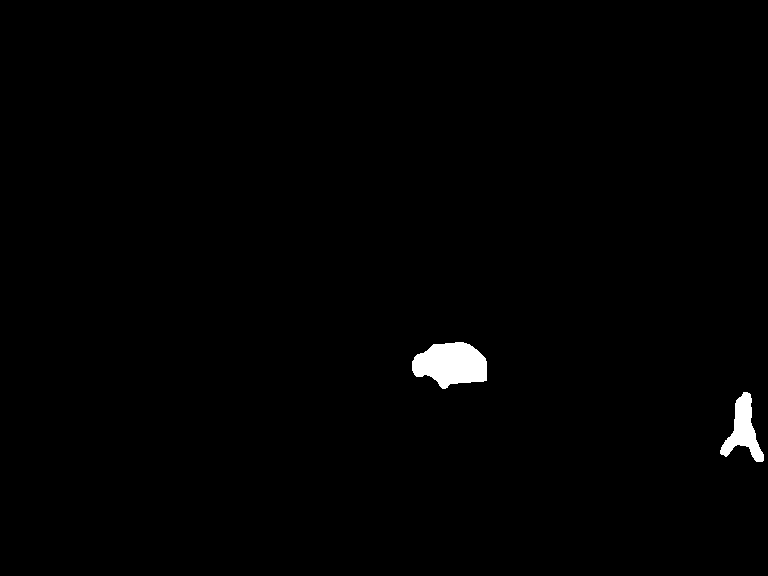
\includegraphics[width=\textwidth]{camGT}
                \caption{Ground truth}
              %  \label{fig:tiger}
        \end{subfigure}
\caption{The spatial sparsity of foreground. A frame from the PETS data set and the corresponding foreground in white. In this example, less than 1\% of the frame is foreground, as N=442,368 and K=3862.  }\label{fig:sparse}
\end{figure}

 \end{frame}


      % -- Frame 3-34 
      \begin{frame}{Compressive Sensing Background Subtraction.}

\begin{algorithm}[H]
\begin{algorithmic}
\REQUIRE Initial compressed background $y^b_0$
\FOR{all t} % \COMMENT{T is the maximum iteration count.}
\STATE Compressively Sense (Encode) $y_t = \Phi x_t$.
\STATE Reconstruct (Decode)   $\hat{x_t} = \Delta (y_t - y^b_t)$
\STATE Update Background  $y^b_{t+1} = \alpha y_{t+1} + (1 - \alpha)y^b_t$
\RETURN  $\boldsymbol{\hat{x_t}}$
\ENDFOR
\end{algorithmic}
\end{algorithm}
\end{frame}


\begin{frame}
  \frametitle{Sparse and Compressible Signals}
  \begin{itemize}
  \item A signal is known as being \textbf{K-sparse} if $\boldsymbol{x} \in R^N$ can be represented as a linear combination of $K$ basis vectors. 
   \item Interested in $K \ll N$.
     \item If a signal is \textbf{compressible} there exist $K$ large coefficients but the remaining $N-K$ coefficients are only required to be small and not necessarily zero. 
  \end{itemize}
 
  \begin{figure}
    \centering
    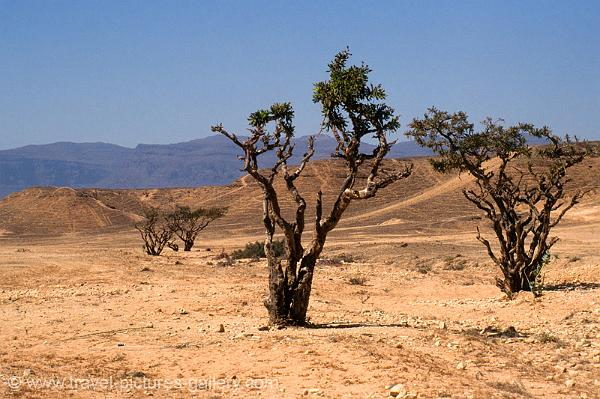
\includegraphics[width = 6cm]{sparseD.jpg}
  \end{figure}

\end{frame}

 \begin{frame}{What is compressive sensing?}
Compressive sensing is a method of \textbf{reducing the amount of data collected} from a signal without compromising the ability to later \textbf{reconstruct the signal accurately.} This method will only work if the signal of interest is compressible. 

\begin{figure}[h]
        \centering
        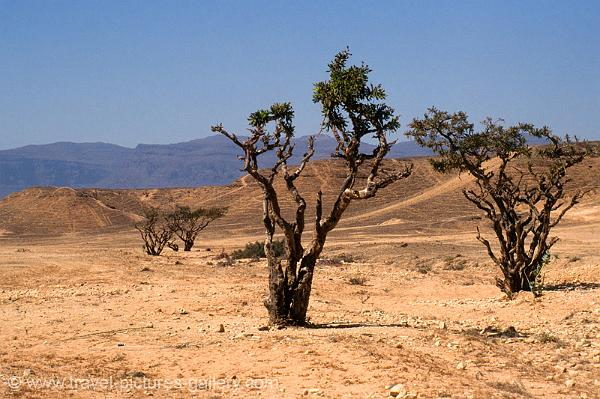
\includegraphics[width = 8cm]{sparseD.jpg}
       \end{figure}

\end{frame}

\begin{frame}{Restricted Isometry Property (RIP)}
 A matrix $\boldsymbol{\Phi}$ satisfies the (RIP) of order $K$ if there exists a $\delta_K  \in (0,1)$ such that 
\begin{equation*}
  \label{eq:40}
  (1 - \delta_k)\|\boldsymbol{x}\|^2_2 \leq\|\boldsymbol{\Phi} \boldsymbol{x}\|^2_2 \leq (1 + \delta_k)\|\boldsymbol{x}\|^2_2,
\end{equation*}

for all $\boldsymbol{x} \in \sum_K = \{\boldsymbol{x}:\|\boldsymbol{x}\|_0 \leq K\} $, \newline

where $\|\boldsymbol{x}\|_0$ is the zero pseudo-norm defined as

\begin{equation*}
\|\boldsymbol{x}\|_0 = \#(i|x_i \neq 0). 
\end{equation*}

If $\boldsymbol{\Phi}$ satisfies the RIP with order $2K$, then $\boldsymbol{\Phi}$ approximately preserves the distance between any pair of $K$-sparse vectors. Unfortunately the task of checking that a matrix satisfies the RIP is a NP-hard problem, but fortunately the RIP will hold true with high probability if $\boldsymbol{\Phi}$ is selected as a random matrix and $M \geq cK\log \frac{N}{K}$, where $c$ is a small constant. 
\end{frame}



\begin{frame}
  \frametitle{Emmanuel Candes}
  \begin{columns}
\begin{column}{.48\textwidth}

  \begin{itemize}
  \item Working with radiologist on MRI. 
  \item Using the phantom image
  \item Found that he could reconstruct the image ``perfectly'' from undersampled data. 
  \item Thought he was fudging. 
   \item Chatted to Terry Tao at pre-school. He thought it was rubbish. 
   \item Sketched out the theory of compressive sensing. 
  \end{itemize}
\end{column}
%\hfill

\begin{column}{.48\textwidth}
  \begin{figure}[h]
   % \centering
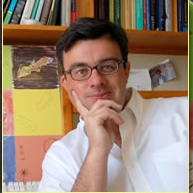
\includegraphics[height = 4cm]{candes.jpg}    

  \end{figure}

\end{column}%
\end{columns}
\end{frame}